\documentclass{article}

% colm-mode: submission (default, anonymous + line numbers)
%             preprint  (non-anonymous, "Preprint. Under review." header)
%             final     (camera-ready, "Published as a conference paper at COLM 2026")
\usepackage[submission]{colm2026_conference}

% colm2026_conference.sty already loads: tgpagella, mathpazo, inconsolata,
%   eso-pic, fancyhdr, natbib (authoryear, round brackets).
% Do NOT reload those here.

% Additional standard packages
\usepackage{microtype}
\usepackage{url}

% Math
\usepackage{amsmath}
\usepackage{amssymb}

% Tables
\usepackage{longtable}
\usepackage{booktabs}
\usepackage{array}     % pandoc uses >{\raggedright\arraybackslash}p{} column types
\usepackage{calc}      % pandoc uses \real{} expressions for column widths
\usepackage{multirow}

% Graphics
\usepackage{graphicx}
\makeatletter
\def\maxwidth{\ifdim\Gin@nat@width>\linewidth\linewidth\else\Gin@nat@width\fi}
\def\maxheight{\ifdim\Gin@nat@height>\textheight\textheight\else\Gin@nat@height\fi}
\def\fps@figure{htbp}
\makeatother

% Code blocks and inline code
\IfFileExists{upquote.sty}{\usepackage{upquote}}{}
\usepackage{fancyvrb}
\newcommand{\passthrough}[1]{#1}

% Line numbers for submission mode (toggled by \ifcolmsubmission in body)
\usepackage{lineno}

% Caption placement — force table captions below (matching CoLM template)
\usepackage{caption}
\captionsetup[table]{position=below}

% hyperref — load after natbib (already loaded by colm sty)
\usepackage{hyperref}
\definecolor{darkblue}{rgb}{0, 0, 0.5}
\hypersetup{colorlinks=true, citecolor=darkblue, linkcolor=darkblue, urlcolor=darkblue}

% pandoc: scale images to fit line width, preserving aspect ratio
\makeatletter
\newsavebox\pandoc@box
\newcommand*\pandocbounded[1]{%
  \sbox\pandoc@box{#1}%
  \Gscale@div\@tempa{\linewidth}{\wd\pandoc@box}%
  \ifdim\@tempa\p@<\p@\scalebox{\@tempa}{\usebox\pandoc@box}\else#1\fi%
}
\makeatother

% pandoc: tight lists
\providecommand{\tightlist}{%
  \setlength{\itemsep}{0pt}\setlength{\parskip}{0pt}}

\title{writeup}

% In submission mode the sty replaces the author block with
% "Anonymous authors / Paper under double-blind review" automatically.
\author{
  \textbf{Zachary Houghton} \\
      Vail Systems, Inc., University of Oregon \\
        \texttt{znhoughton@ucdavis.edu}
    }

\begin{document}

% Enable line numbers in submission mode
\ifcolmsubmission
\linenumbers
\fi

\maketitle

\begin{abstract}
(Abstract goes here.)
\end{abstract}

\section{Introduction}\label{introduction}

\section{Model Training}\label{model-training}

In order to examine the representation of binomials in language models,
we trained six autoregressive language models from scratch using the OPT
architecture \citep{zhangOPTOpenPretrained2022}, crossing two training
corpora with three model sizes (125M, 350M, and 1.3B parameters), for a
total of six models. All models share a common tokenizer: a Byte-Pair
Encoding (BPE) tokenizer with a vocabulary of 8,192 tokens and a context
window of 1,024 tokens, trained once on the full BabyLM corpus and
reused across all six models to ensure that differences between models
reflect training data and scale rather than tokenization. Models were
trained on two NVIDIA H100 GPUs using PyTorch Distributed Data Parallel
(DDP) in bfloat16 precision, with AdamW optimization and a linear
learning rate schedule with 4,000 warmup steps.

The first corpus that we trained the models on was BabyLM\citep[Version
3,][]{charpentier2025babylmturns3}, a developmentally plausible corpus
of approximately 150M tokens consisting of child-directed speech
(CHILDES), children's books, and simple web text. Each model was trained
for 64 epochs over this corpus, yielding approximately 9.1B total
training tokens. The second corpus was a 10B-token subset of C4
\citep{raffelExploringLimitsTransfer2020}, a filtered English web text
corpus. C4 models were trained for a single pass over this corpus, also
yielding approximately 10B training tokens. Comparing the two corpora
allows us to examine how the content and diversity of the training data
shapes the learning of binomials in language models.

Checkpoints were saved approximately every 10M tokens throughout
training and pushed to HuggingFace Hub, giving us dense coverage of each
model's learning trajectory. All models and checkpoints will be made
publicly available.\footnote{The huggingface account would reveal the
  identity of one of the authors and is thus omitted from the
  double-blind review phase.} Table~\ref{tbl-models} summarizes the key
training parameters for each model.

\begin{longtable}[]{@{}lrrrr@{}}

\toprule\noalign{}
Corpus & Params & Total tokens & Checkpoints & LR \\
\midrule\noalign{}
\endhead
\bottomrule\noalign{}
\endlastfoot
BabyLM & 125M & \textasciitilde9.1B & \textasciitilde910 &
\(3\times10^{-4}\) \\
BabyLM & 350M & \textasciitilde9.1B & \textasciitilde910 &
\(1\times10^{-4}\) \\
BabyLM & 1.3B & \textasciitilde9.1B & \textasciitilde860 &
\(1\times10^{-4}\) \\
C4 & 125M & \textasciitilde10B & \textasciitilde1,010 &
\(3\times10^{-4}\) \\
C4 & 350M & \textasciitilde10B & \textasciitilde1,005 &
\(1\times10^{-4}\) \\
C4 & 1.3B & \textasciitilde10B & \textasciitilde960 &
\(1\times10^{-4}\) \\


\caption{\label{tbl-models}Training configuration for all six models.
All models use the OPT architecture, a shared BPE tokenizer (vocab
8,192; context 1,024 tokens), AdamW optimization, and a linear LR
schedule with 4,000 warmup steps.}

\tabularnewline
\end{longtable}

All six models showed smooth convergence in training loss throughout
training, starting near the theoretical random baseline
(\(\ln 8192 \approx 9.01\)) and decreasing consistently. Held-out
validation perplexity confirmed successful training for all models; full
loss curves and perplexity figures are reported in Appendix
\ref{sec-training-quality}. Notably, the BabyLM 1.3B model showed
elevated final validation perplexity relative to the 350M model (2,557
vs.~290), consistent with mild overfitting given the small corpus
(approximately 150M tokens) --- unsurprising for a 1.3B parameter model
trained on such limited data. We return to the implications of this for
our main analyses in the Results.

\section{Binomial Ordering
Preferences}\label{binomial-ordering-preferences}

In this section we present three complementary analyses examining how
our models represent binomial ordering preferences over the course of
training. The first analysis examines raw \textbf{preference} (how
strongly each model favors the alphabetically ordered form of a
binomial). The second examines the \textbf{signed gap} (the extent to
which models' preferences deviate from what corpus frequency alone would
predict). The third examines \textbf{deviation from corpus predictions}
as a function of training, examining how the ordering preferences of
models deviates from its training distribution as a function of
learning.

\subsection{Preference}\label{preference}

In this section, we examine whether our models learn binomial ordering
preferences, and if so what factors predict that preference. For each
model checkpoint and binomial pair, we compute the model's ordering
\textbf{preference} as the difference in log-probability of the
alphabetically ordered form (e.g., \emph{bread and butter}) compared to
the non-alphabetically ordered form (e.g., \emph{butter and bread}). The
alphabetical form is used as a relatively neutral baseline
\citep[following][]{morgan2016abstractknowledgedirect}. Concretely, for
a binomial with alphabetically ordered token sequence \(s_\alpha\) and
non-alphabetically ordereed \(s_n\):

\[\text{preference}_i = \log P_\theta(s_{\alpha,i}) - \log P_\theta(s_{n,i})\]

where \(\log P_\theta(s)\) is the summed log-probability of sequence
\(s\) under model parameters \(\theta\). Positive values indicate that
the model assigns higher probability to the alphabetically ordered form.

We regress preference on three item-level predictors using a Bayesian
mixed-effects regression model \citep{burknerBrmsPackageBayesian2017}.
\textbf{Generative Preference} (GenPref) is an estimate of ordering
preferences driven by a combination of phonological and semantic
predictors \citep{morgan2016abstractknowledgedirect}. \textbf{RelFreq}
is the relative corpus frequency of the alphabetically ordered form
(centered):

\[\text{RelFreq}_i = P(\text{alpha})_i - 0.5, \quad \text{where} \quad P(\text{alpha})_i = \frac{c_{\alpha,i}}{c_{\alpha,i} + c_{n,i}}\]

and \(c_{\alpha,i}\), \(c_{n,i}\) are the corpus counts of the
alpha-ordered and non-alphabetical forms of binomial \(i\),
respectively. \textbf{Log total frequency} is
\(\ln(c_{\alpha,i} + c_{n,i})\), the natural log of total corpus
occurrences of the binomial in either order, centered. We include
interaction terms for GenPref and log total frequency as well as RelFreq
and log total frequency, allowing the model to capture how ordering
preferences may be differently affected by GenPref and RelFreq depending
on the overall frequency of that binomial:

\[\text{preference} \sim \text{GenPref} \times \ln(\text{total}) + \text{RelFreq} \times \ln(\text{total}) + (1 \mid \text{binomial})\]

We fit this model at the final training checkpoint and at 20
evenly-spaced checkpoints throughout training to examine the learning
trajectory of binomial ordering preferences. We additionally fit a
checkpoint-interacted model in which training stage (tokens encountered,
scaled and centered) is included as a predictor to test whether effects
grow or shrink linearly over training:

\[\text{preference} \sim (\text{GenPref} + \text{RelFreq} + \ln(\text{total})) \times \text{tokens} + (1 \mid \text{binomial})\]

\subsubsection{Results}\label{results}

\paragraph{Final Checkpoint}\label{final-checkpoint}

The results of the Bayesian mixed-effects regression at the final
checkpoint are presented in Table~\ref{tbl-pref-final} and visualized in
Figure~\ref{fig-pref-final-coefs}. The results suggest that relative
frequency is a credible predictor of the model's ordering preferences
across all six models, which is consistent with models' ordering
preferences being at least partly driven by the distributional
statistics of their training data. Interestingly, the effect of GenPref
shows a graded pattern across model sizes, with the 125M parameter
models showing a credible positive effect, the 350M models showing a
somewhat weaker effect, and the 1.3B models showing little credible
evidence of a GenPref effect.

\begin{figure}

\centering{

\pandocbounded{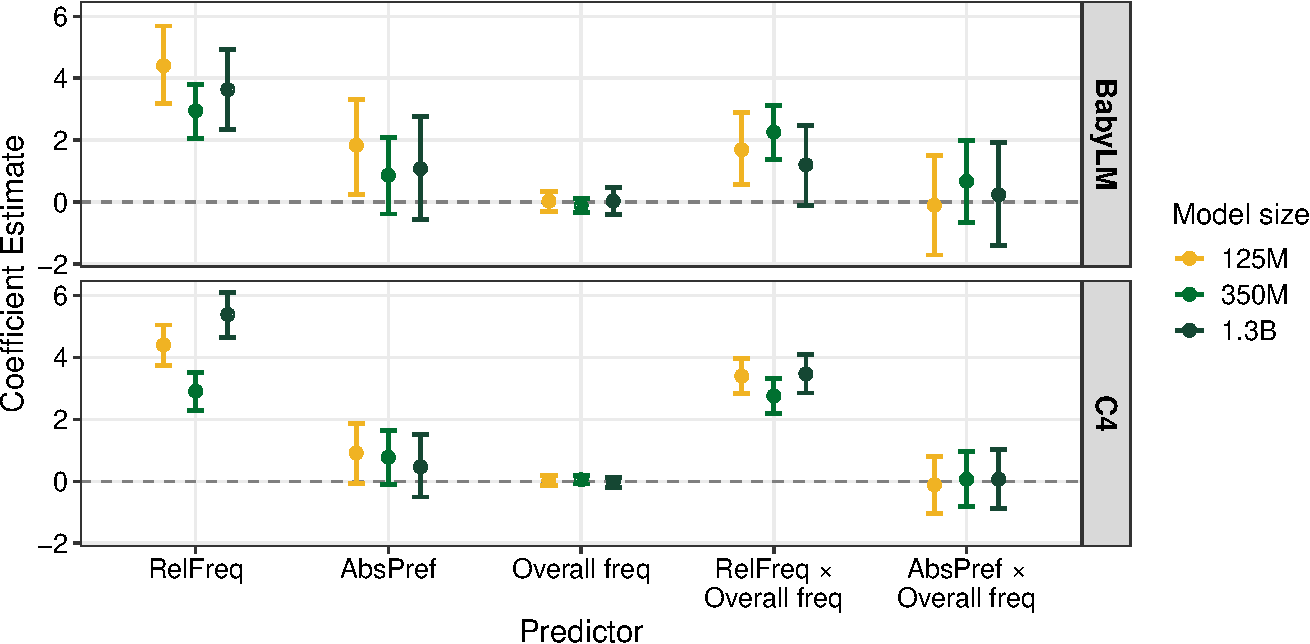
\includegraphics[keepaspectratio]{writeup_files/figure-pdf/fig-pref-final-coefs-1.pdf}}

}

\caption{\label{fig-pref-final-coefs}Posterior fixed-effect estimates
for predictors of raw preference at the final training checkpoint. Error
bars show 95\% credible intervals.}

\end{figure}%

\paragraph{GenPref Significance Over
Training}\label{genpref-significance-over-training}

The results from Figure~\ref{fig-pref-traj-sig} suggest a size-graded
pattern across the BabyLMs, with smaller models showing credible GenPref
effects from early in training while larger models show weaker effects
throughout training. Interestingly, the C4-trained 1.3B model shows a
credible GenPref effect early in training that attenuates with further
exposure, suggesting that the learning of generative preferences may
depend on an interaction between model scale and the volume and
diversity of the training data.

\begin{figure}

\centering{

\pandocbounded{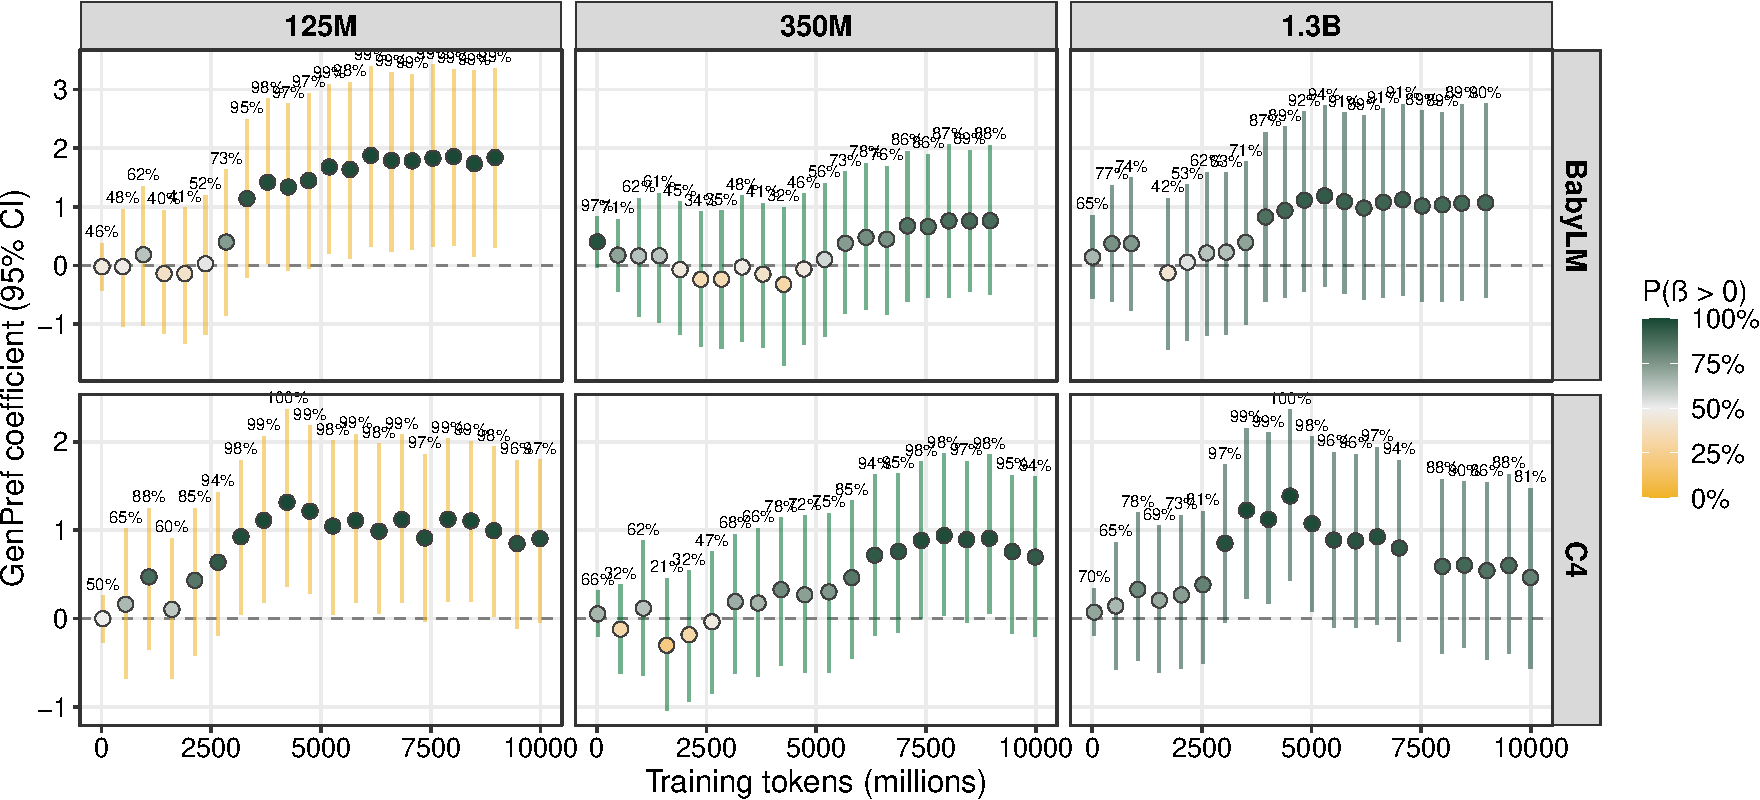
\includegraphics[keepaspectratio]{writeup_files/figure-pdf/fig-pref-traj-sig-1.pdf}}

}

\caption{\label{fig-pref-traj-sig}GenPref coefficient (95\% CI) at each
of 20 sampled training checkpoints, for raw preference models. Point
fill encodes P(\(\beta\) \textgreater{} 0): green indicates the
posterior is predominantly positive, gold predominantly negative, grey
uncertain.}

\end{figure}%

\paragraph{Checkpoint-Interacted
Model}\label{checkpoint-interacted-model}

The results of the checkpoint-interacted model are presented in
Table~\ref{tbl-pref-ckpt} and visualized in
Figure~\ref{fig-pref-ckpt-coefs}. Because all predictors are centered,
main effects in this model reflect the estimated influence of each
predictor at the midpoint of training. In other words, the main effects
of GenPref and RelFreq reflect their respective influences halfway
through training, while interactions with training stage indicate
whether each effect grows or shrinks linearly over the course of
training.

The results suggest that there is an effect of relative frequency across
all six models at the training midpoint, and that this effect grows
stronger as training progresses. Interestingly, the GenPref results
differ across corpora and model sizes. Among the BabyLM models, the
results suggest that only the 125M model shows an effect of GenPref at
the training midpoint, and that this effect grows further over the
course of training, while the 350M and 1.3B BabyLM models show little
credible evidence of a GenPref effect. Among the C4 models, the results
suggest that all three models show a credible GenPref effect at the
training midpoint, though this effect appears to be weakest for the 350M
model.

\begin{figure}

\centering{

\pandocbounded{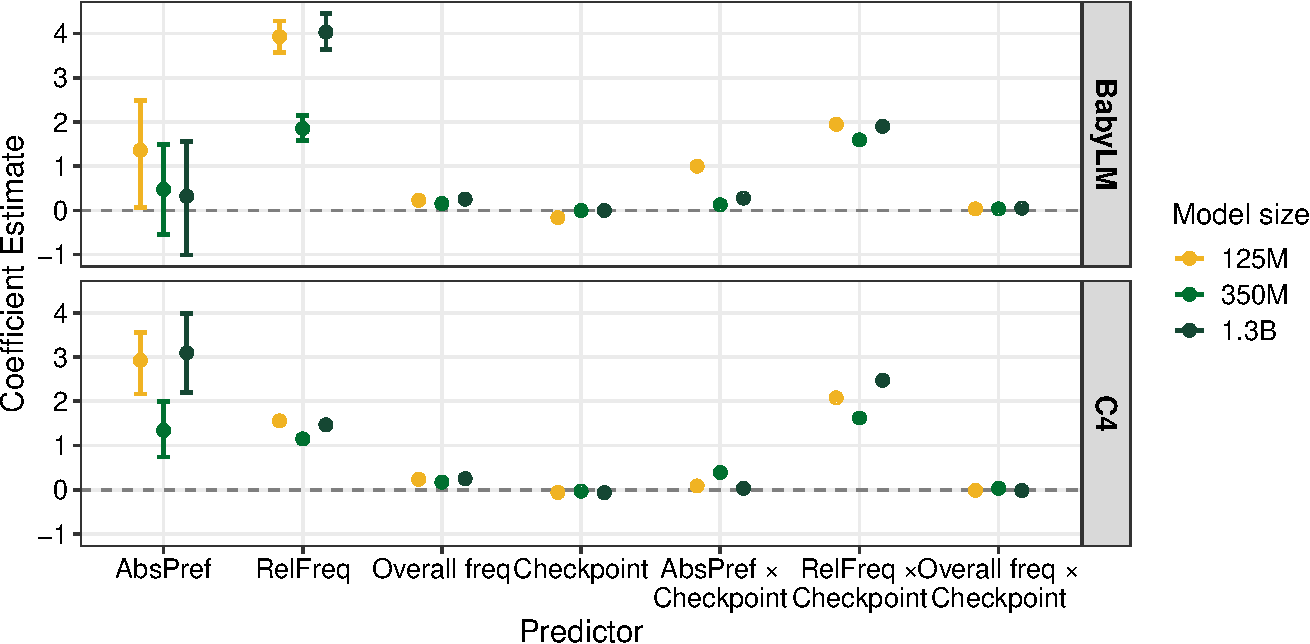
\includegraphics[keepaspectratio]{writeup_files/figure-pdf/fig-pref-ckpt-coefs-1.pdf}}

}

\caption{\label{fig-pref-ckpt-coefs}Posterior fixed-effect estimates
from the checkpoint-interacted preference model. Interactions with
training stage (tokens, z-scored) test whether each predictor's effect
on raw preference changes linearly over the course of training.}

\end{figure}%

\subsection{Signed Gap}\label{signed-gap}

Since we have access to the exact training data each model encountered,
we are able to calculate exactly how many times the model has seen each
ordering of each binomial at each checkpoint. Thus, in this section, we
examine the \textbf{signed gap}: the difference between each model's
preference score and the log corpus frequency ratio for that binomial.
Formally:

\[\text{signed gap}_i = \text{preference}_i - \ln\frac{c_{\alpha,i}}{c_{n,i}}\]

where \(\text{preference}_i\) is defined as above and
\(c_{\alpha,i} / c_{n,i}\) is the corpus frequency ratio of the
alphabetically ordered to the non-alphabetical form. A signed gap of
zero means the model's preference exactly matches what corpus frequency
predicts; positive values indicate a stronger preference for alpha order
than corpus statistics would suggest, and negative values the reverse.
Using the signed gap as the outcome allows us to ask whether models
develop ordering preferences that go beyond simply reflecting the
distributional statistics of their training data. We regress signed gap
on the same predictors as the preference model:

\[\text{signed gap} \sim \text{GenPref} \times \ln(\text{total}) + \text{RelFreq} \times \ln(\text{total}) + (1 \mid \text{binomial})\]

We fit this model at the final checkpoint and at 20 evenly-spaced
checkpoints throughout training. We additionally fit a
checkpoint-interacted model to test whether the effect of each predictor
grows or shrinks linearly over training:

\[\text{signed gap} \sim (\text{GenPref} + \text{RelFreq} + \ln(\text{total})) \times \text{tokens} + (1 \mid \text{binomial})\]

\subsubsection{Results}\label{results-1}

\paragraph{Final Checkpoint}\label{final-checkpoint-1}

The results of the Bayesian mixed-effects regression for signed gap at
the final checkpoint are presented in Table~\ref{tbl-sg-final} and
visualized in Figure~\ref{fig-sg-final-coefs}. Recall that because the
signed gap removes the contribution of corpus frequency from the
preference score, a credible positive effect of GenPref here would
suggest that models develop ordering preferences consistent with
phonological and semantic biases over and above what the training corpus
frequency ratio would predict. A positive effect of relative frequency,
on the other hand, would indicate that the model's ordering preference
for the alphabetically ordered form is more extreme than the training
data alone would predict, while a negative effect would indicate the
opposite.

The results for relative frequency are quite mixed across model sizes
and corpora. Among the BabyLM models, the largest model shows a negative
effect of relative frequency, while the two smaller models show little
to no effect. Among the C4 models, the pattern is reversed: the two
smaller models show a negative effect of relative frequency, while the
largest shows little evidence of an effect. In terms of generative
preferences, the 125M BabyLM model shows a weak positive effect of
GenPref, while the two larger BabyLM models show little evidence of an
effect. For the C4 models, the pattern is similar: the 125M C4 model
shows a possible effect of GenPref (approximately 89\% of posterior
samples were greater than zero), while the two larger C4 models show
little evidence of an effect.

Taken together, the signed gap results suggest that models' ordering
preferences are broadly consistent with what corpus frequency predicts,
with limited evidence of preferences that go beyond the training
distribution. Interestingly, the modest GenPref effects that do appear
are consistently concentrated in the smallest models across both
corpora, suggesting that smaller models may be more sensitive to
abstract ordering biases even when controlling for frequency.

\begin{figure}

\centering{

\pandocbounded{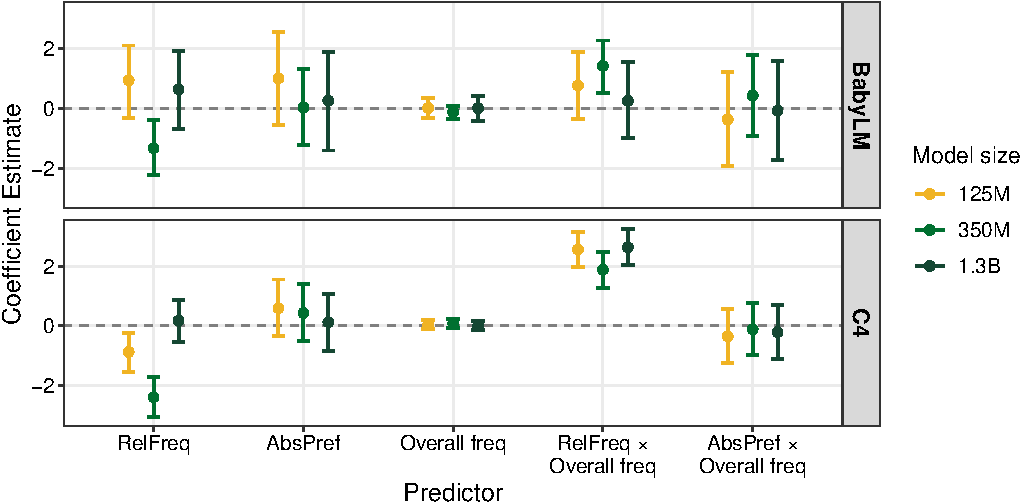
\includegraphics[keepaspectratio]{writeup_files/figure-pdf/fig-sg-final-coefs-1.pdf}}

}

\caption{\label{fig-sg-final-coefs}Posterior fixed-effect estimates for
predictors of signed gap (preference minus log corpus frequency ratio)
at the final training checkpoint. Error bars show 95\% credible
intervals.}

\end{figure}%

\paragraph{GenPref Significance Over
Training}\label{genpref-significance-over-training-1}

The results from Figure~\ref{fig-sg-traj-sig} largely mirror the
preference trajectory in Figure~\ref{fig-pref-traj-sig}. The 125M models
show a steady increase in the GenPref coefficient over training
regardless of corpus, while the two larger BabyLM models show little to
no effect of GenPref throughout. Interestingly, the two larger C4 models
do show some evidence of a GenPref effect over training, suggesting that
training data diversity may play a role in the learning of generative
preferences. Additionally, as was the case in the preference trajectory,
the largest C4 model shows a U-shaped pattern, with the GenPref effect
initially growing before subsequently declining.

\begin{figure}

\centering{

\pandocbounded{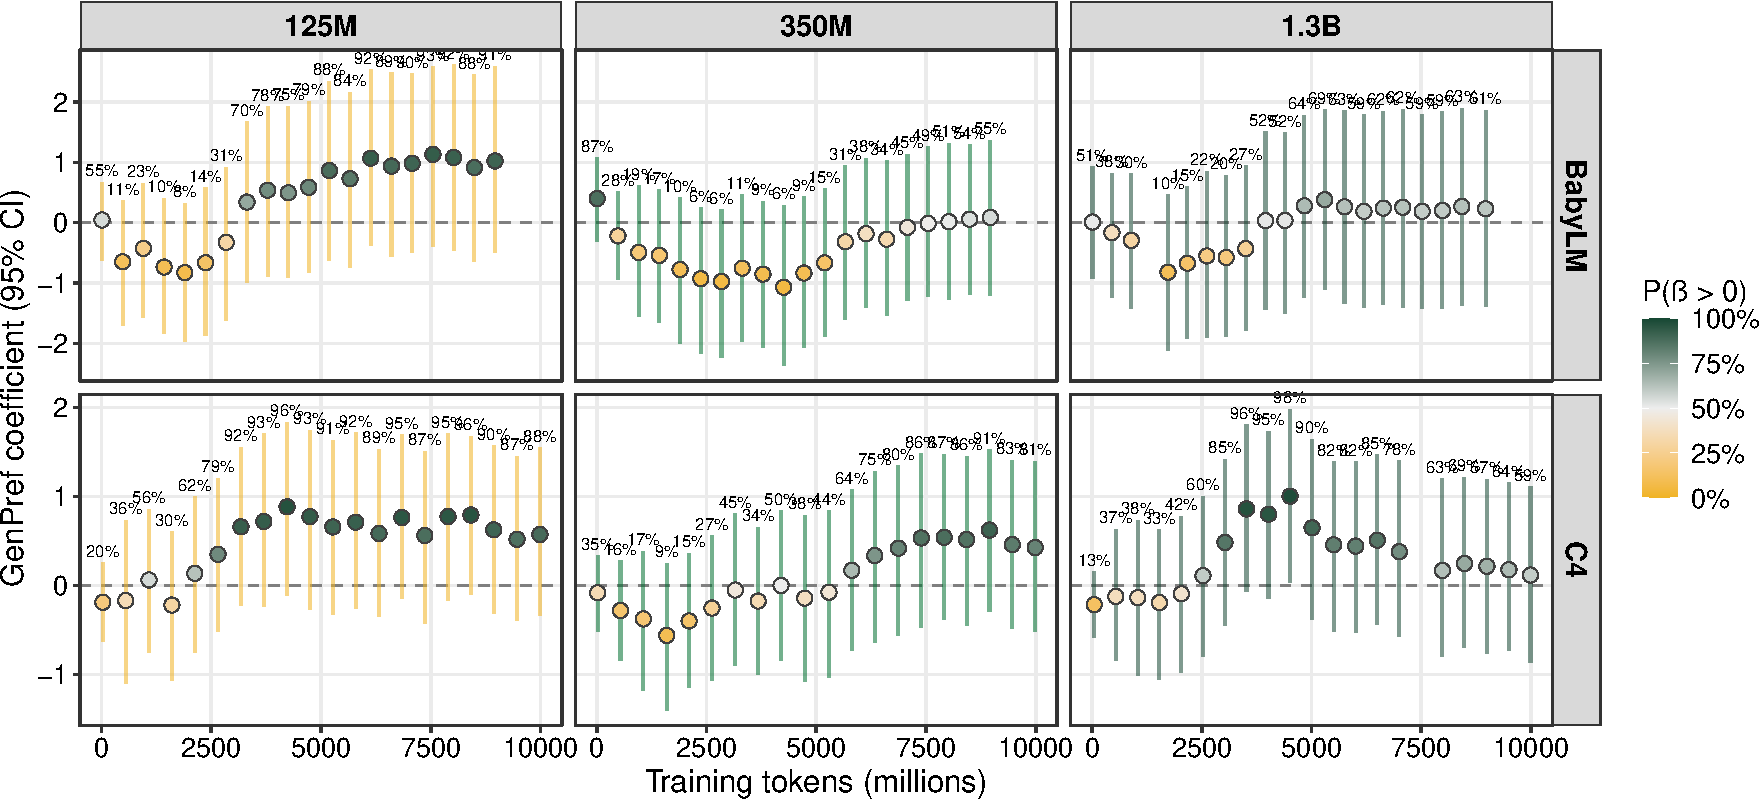
\includegraphics[keepaspectratio]{writeup_files/figure-pdf/fig-sg-traj-sig-1.pdf}}

}

\caption{\label{fig-sg-traj-sig}GenPref coefficient (95\% CI) at each of
20 sampled training checkpoints, for signed gap models. Point fill
encodes P(\(\beta\) \textgreater{} 0): green indicates the posterior is
predominantly positive, gold predominantly negative, grey uncertain.}

\end{figure}%

\paragraph{Checkpoint-Interacted
Model}\label{checkpoint-interacted-model-1}

The results of the checkpoint-interacted signed gap model are presented
in Table~\ref{tbl-sg-ckpt} and visualized in
Figure~\ref{fig-sg-ckpt-coefs}. Among the BabyLM models, the results
suggest that the 125M model shows a credible effect of GenPref at the
training midpoint, and that this effect grows stronger as training
progresses. The negative effect of relative frequency across all three
BabyLM models suggests that, at the midpoint of training, the models'
preferences for the alphabetically ordered form fall short of what
corpus frequency alone would predict, and that this gap narrows over the
course of training (given the positive interaction effect between
relative frequency and checkpoint). For the C4 models, the 125M and 1.3B
models show an effect of GenPref, while the 350M model does not. The C4
models show a similar pattern for relative frequency as the BabyLM
models, with a negative effect that also narrows over training.

\begin{figure}

\centering{

\pandocbounded{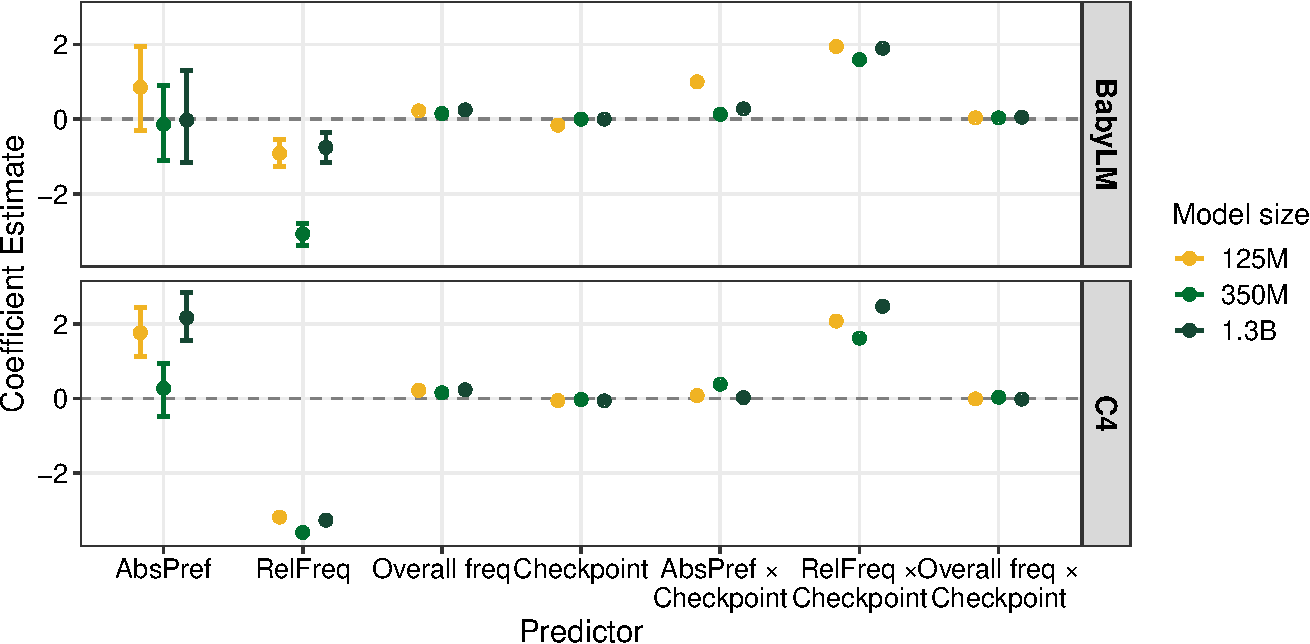
\includegraphics[keepaspectratio]{writeup_files/figure-pdf/fig-sg-ckpt-coefs-1.pdf}}

}

\caption{\label{fig-sg-ckpt-coefs}Posterior fixed-effect estimates from
the checkpoint-interacted signed gap model.}

\end{figure}%

\subsection{Deviation from Corpus
Predictions}\label{deviation-from-corpus-predictions}

In this section, we examine how closely models track corpus-frequency
predictions over the course of training, using two descriptive summaries
and one regression model. First, we compute the \textbf{mean absolute
signed gap} across all binomials at each checkpoint
(Figure~\ref{fig-abs-signed-gap}):

\[\overline{|\text{signed gap}|}_t = \frac{1}{N}\sum_{i=1}^{N} \left|\text{signed gap}_{i,t}\right|\]

where \(t\) indexes the checkpoint and \(N\) is the number of binomials.
Lower values indicate that models' preferences are, on average, closer
to what corpus frequency would predict. Second, we compute the
\textbf{Pearson correlation between model preference and log corpus
frequency ratio} across items at each checkpoint
(Figure~\ref{fig-freq-tracking}):

\[r_t = \mathrm{Cor}\!\left(\text{preference}_{i,t},\; \ln\frac{c_{\alpha,i}}{c_{n,i}}\right)\]

Values near 1 indicate near-perfect frequency tracking. Finally, we fit
a model predicting the absolute signed gap from training stage and log
total frequency to test whether models become more or less corpus-like
as training progresses and whether this depends on item frequency
(Figure~\ref{fig-absgap-coefs}; Table~\ref{tbl-absgap}):

\[|\text{signed gap}| \sim \text{tokens} \times \ln(\text{total}) + (1 \mid \text{binomial})\]

\subsubsection{Results}\label{results-2}

The results from Figure~\ref{fig-abs-signed-gap} suggest that the mean
absolute signed gap grows throughout training for all six models,
indicating that models' ordering preferences deviate more from what
corpus frequency alone would predict as training progresses. Among the
BabyLM models, this growth is most pronounced for the 1.3B model and
weakest for the 350M model. Among the C4 models, all three follow a
broadly similar trajectory.

Interestingly, Figure~\ref{fig-freq-tracking} suggests that even as the
absolute signed gap grows over training, models' ordering preferences
simultaneously become more correlated with corpus frequency. In other
words, models' preferences grow more extreme over training, but in a
direction that is broadly consistent with the corpus frequency ordering.

Finally, the results of the Bayesian mixed-effects regression are
presented in Table~\ref{tbl-absgap} and visualized in
Figure~\ref{fig-absgap-coefs}. The effect of training stage on absolute
signed gap is quite mixed across models. Among the BabyLM models, the
125M and 1.3B models show a positive effect, while the 350M model shows
a negative effect. Among the C4 models, the two smaller models show a
slightly negative effect while the largest shows a slightly positive
effect. In general, the effect of training stage appears weaker for the
C4 models than for the BabyLM models, suggesting that training data
diversity may dampen the growth of the gap between models' learned
preferences and what corpus frequency alone predicts.

The effect of overall frequency also varies across models. The 125M and
1.3B BabyLM models show a slightly negative effect of overall frequency,
suggesting that the absolute signed gap is smaller for more frequently
encountered binomials, while the 350M BabyLM model shows a large
positive effect, suggesting the opposite. All three C4 models show a
strong positive effect of overall frequency, indicating that the gap
between model preference and the frequency-based prediction is larger
for higher-frequency binomials. This pattern is of particular interest
given existing work demonstrating frequency-dependent preference
extremity in humans, whereby humans develop more extreme ordering
preferences for high-frequency binomials over time
\citep[e.g.,][]{morganFrequencydependentRegularizationIterated2016a, houghton2024frequencydependentpreferenceextremity, houghton2025boltsnutslanguage}.
The present results suggest that model size and training data diversity
may modulate a similar effect in language models, though a full
investigation of this question is left for future research.

\begin{figure}

\centering{

\pandocbounded{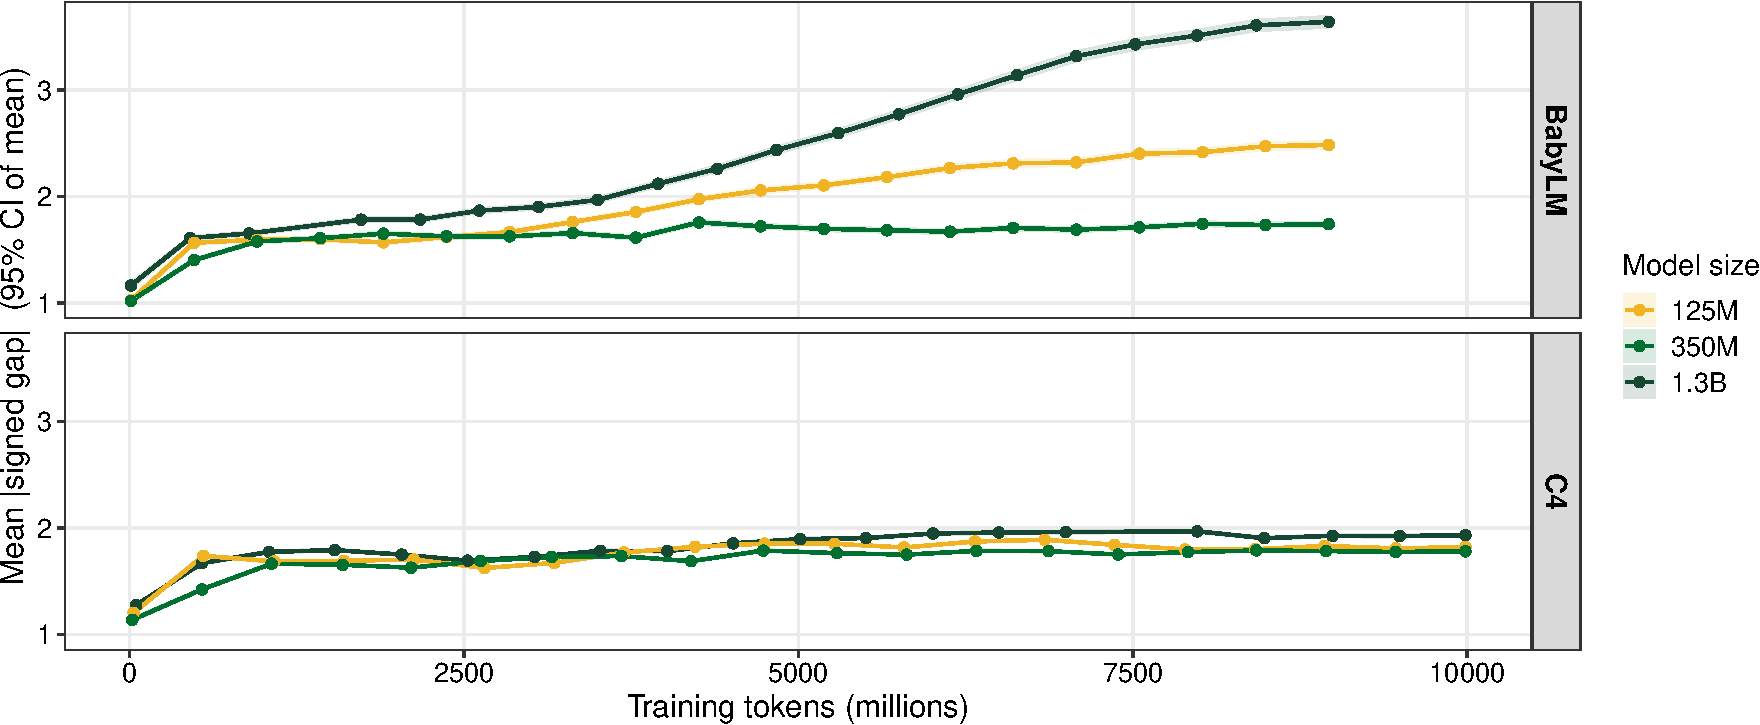
\includegraphics[keepaspectratio]{writeup_files/figure-pdf/fig-abs-signed-gap-1.pdf}}

}

\caption{\label{fig-abs-signed-gap}Mean absolute signed gap across items
at each of 20 sampled checkpoints. Higher values indicate that models'
preference magnitudes deviate more from what corpus frequency predicts,
on average.}

\end{figure}%

\begin{figure}

\centering{

\pandocbounded{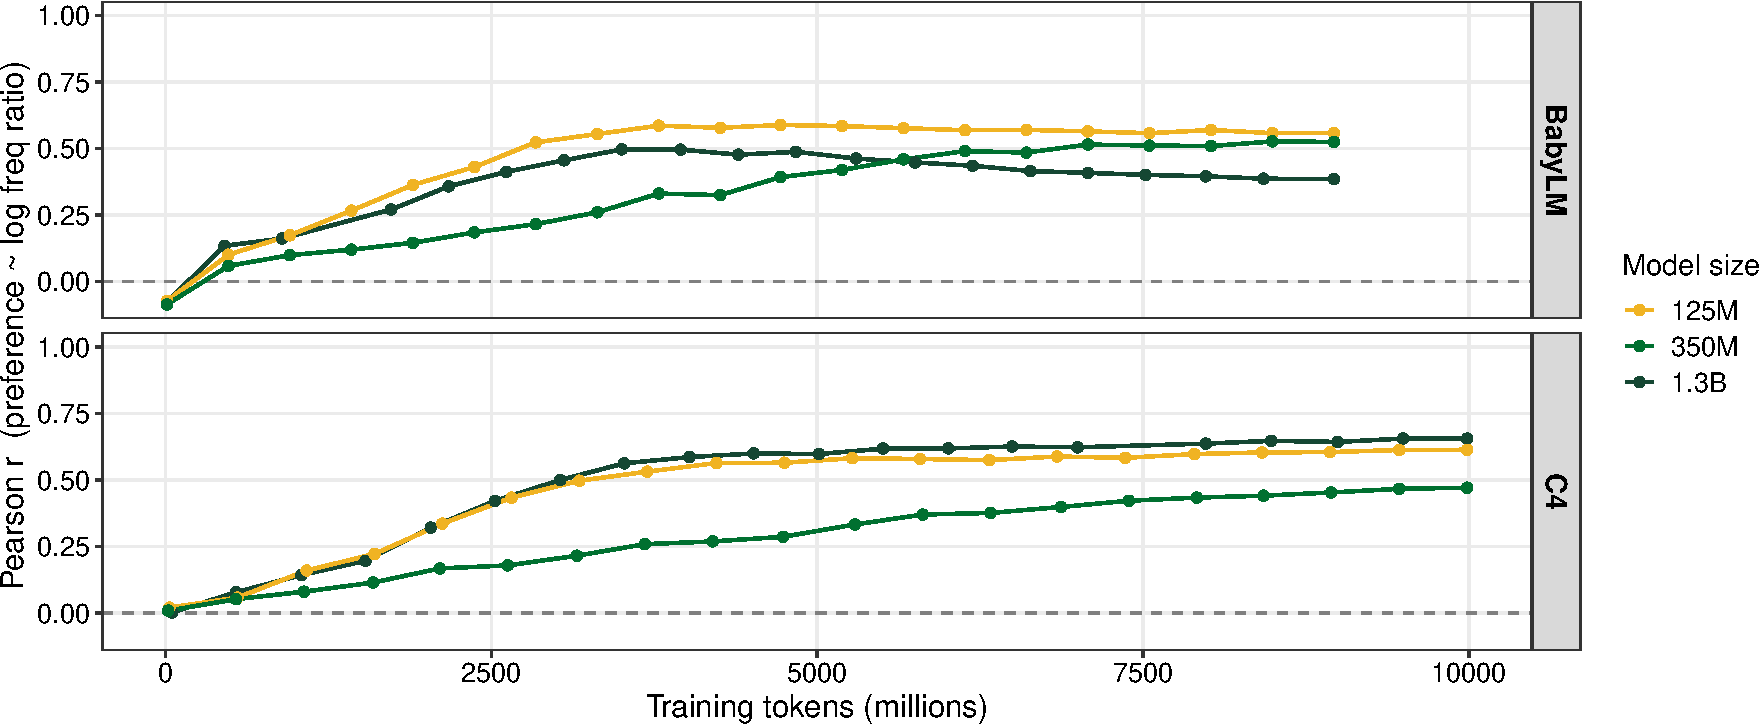
\includegraphics[keepaspectratio]{writeup_files/figure-pdf/fig-freq-tracking-1.pdf}}

}

\caption{\label{fig-freq-tracking}Pearson correlation between model
preference and log corpus frequency ratio across items at each sampled
checkpoint. Values near 1 indicate that models rank binomials by
preference in the same order as the corpus frequency ratio.}

\end{figure}%

\begin{figure}

\centering{

\pandocbounded{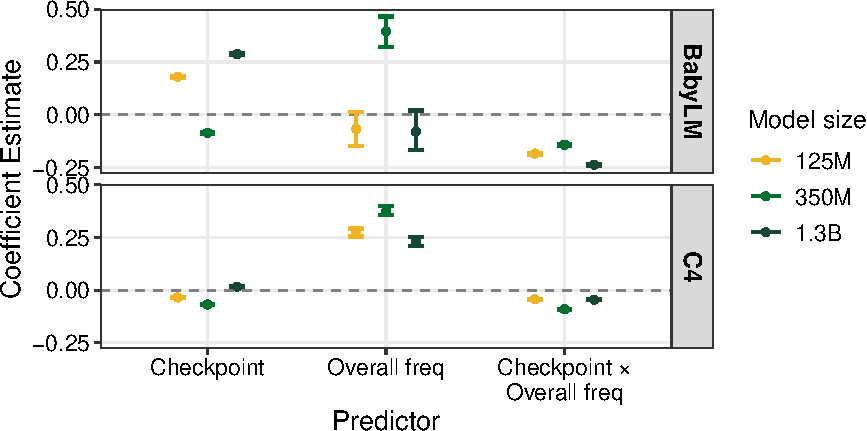
\includegraphics[keepaspectratio]{writeup_files/figure-pdf/fig-absgap-coefs-1.pdf}}

}

\caption{\label{fig-absgap-coefs}Posterior fixed-effect estimates for
predictors of absolute signed gap. The main effect of training stage
(tokens, z) captures overall growth or shrinkage in preference
magnitude; the interaction tests whether this depends on item-level
corpus exposure.}

\end{figure}%

\section{Discussion}\label{discussion}

The results of the present study suggest that the models trained here do
develop binomial ordering preferences over the course of training, and
that these preferences are at least partly driven by the distributional
statistics of the training data. Beyond frequency, however, the picture
is more nuanced. Smaller models --- particularly the 125M models across
both corpora --- show the most consistent evidence of GenPref effects,
suggesting that they are sensitive to abstract ordering preferences over
and above what corpus frequency alone would predict. Larger models, by
contrast, show weaker or absent GenPref effects at the final checkpoint,
though the trajectory results suggest that these models do show some
sensitivity to GenPref earlier in training, with the effect weakening as
training progresses. This may reflect a tendency for larger models to
gradually shift toward relying on distributional frequency as they
accumulate more training experience, at the expense of abstract
knowledge. The nature of the training corpus also appears to matter:
C4-trained models generally show weaker deviations from corpus frequency
predictions than BabyLM-trained models, suggesting that training data
diversity plays a role in shaping models' ordering preferences. Finally,
as training progresses, models' preferences grow more extreme in a
direction broadly consistent with corpus frequency, but the absolute gap
between model preferences and frequency-based predictions also grows,
with the size of this gap modulated by both model size and item
frequency in a manner reminiscent of frequency-dependent preference
extremity observed in humans.

\section{Conclusion}\label{conclusion}

\bibliography{references}
\bibliographystyle{colm2026_conference}

\appendix

\section{Training Quality}\label{sec-training-quality}

\begin{longtable}[]{@{}lrrr@{}}

\toprule\noalign{}
Corpus & Params & Initial PPL & Final PPL \\
\midrule\noalign{}
\endhead
\bottomrule\noalign{}
\endlastfoot
BabyLM & 125M & 9725 & 537.50 \\
BabyLM & 350M & 9470 & 289.68 \\
BabyLM & 1.3B & 13078 & 2557.08 \\
C4 & 125M & 9528 & 31.63 \\
C4 & 350M & 9352 & 43.16 \\
C4 & 1.3B & 12275 & 27.87 \\


\caption{\label{tbl-perplexity}Perplexity at initialization and final
checkpoint for all six models. Perplexity = \(e^{\text{loss}}\); initial
perplexity is derived from the first logged training step; final
perplexity is measured on a held-out validation set (first 5\% of BabyLM
training split for BabyLM models; official C4 validation split for C4
models). The BabyLM 1.3B model's elevated final perplexity relative to
350M reflects overfitting pressure on a small corpus.}

\tabularnewline
\end{longtable}

\begin{figure}

\centering{

\pandocbounded{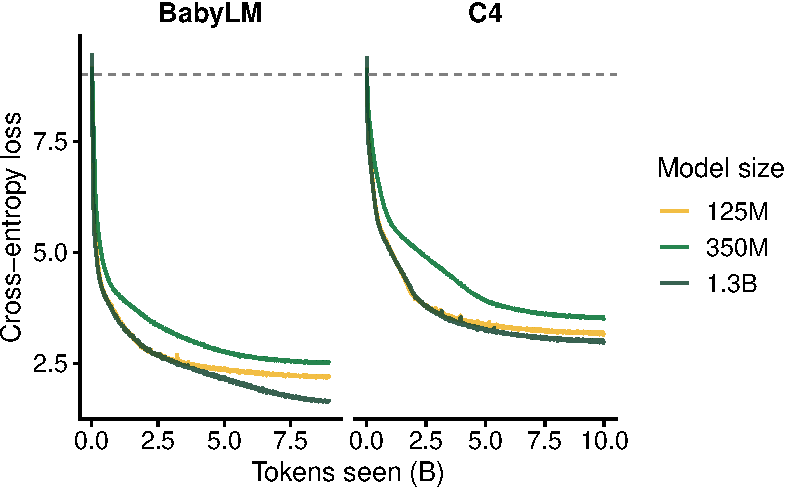
\includegraphics[keepaspectratio]{writeup_files/figure-pdf/fig-loss-curves-1.pdf}}

}

\caption{\label{fig-loss-curves}Training loss over the course of
training for all six models, separated by corpus. All models start near
the theoretical random baseline (\(\ln 8192 \approx 9.01\)) and converge
smoothly; the 1.3B model achieves the lowest final loss in both
corpora.}

\end{figure}%

\section{Posterior Coefficient
Tables}\label{posterior-coefficient-tables}

\subsection{Preference: Final
Checkpoint}\label{preference-final-checkpoint}

\begin{longtable}[]{@{}
  >{\raggedright\arraybackslash}p{(\linewidth - 14\tabcolsep) * \real{0.0843}}
  >{\raggedright\arraybackslash}p{(\linewidth - 14\tabcolsep) * \real{0.0602}}
  >{\raggedright\arraybackslash}p{(\linewidth - 14\tabcolsep) * \real{0.3614}}
  >{\raggedleft\arraybackslash}p{(\linewidth - 14\tabcolsep) * \real{0.0843}}
  >{\raggedleft\arraybackslash}p{(\linewidth - 14\tabcolsep) * \real{0.0723}}
  >{\raggedleft\arraybackslash}p{(\linewidth - 14\tabcolsep) * \real{0.0843}}
  >{\raggedleft\arraybackslash}p{(\linewidth - 14\tabcolsep) * \real{0.0723}}
  >{\raggedleft\arraybackslash}p{(\linewidth - 14\tabcolsep) * \real{0.1807}}@{}}

\toprule\noalign{}
\begin{minipage}[b]{\linewidth}\raggedright
Corpus
\end{minipage} & \begin{minipage}[b]{\linewidth}\raggedright
Size
\end{minipage} & \begin{minipage}[b]{\linewidth}\raggedright
Term
\end{minipage} & \begin{minipage}[b]{\linewidth}\raggedleft
Mean
\end{minipage} & \begin{minipage}[b]{\linewidth}\raggedleft
SD
\end{minipage} & \begin{minipage}[b]{\linewidth}\raggedleft
2.5\%
\end{minipage} & \begin{minipage}[b]{\linewidth}\raggedleft
97.5\%
\end{minipage} & \begin{minipage}[b]{\linewidth}\raggedleft
\(P(\beta > 0)\)
\end{minipage} \\
\midrule\noalign{}
\endhead
\bottomrule\noalign{}
\endlastfoot
BabyLM & 125M & GenPref & 1.835 & 0.790 & 0.243 & 3.313 & 0.990 \\
BabyLM & 125M & GenPref \(\times\) Overall freq & -0.105 & 0.827 &
-1.713 & 1.514 & 0.449 \\
BabyLM & 125M & Overall freq (ln total) & 0.024 & 0.170 & -0.312 & 0.339
& 0.556 \\
BabyLM & 125M & RelFreq \(\times\) Overall freq & 1.688 & 0.587 & 0.553
& 2.892 & 0.998 \\
BabyLM & 125M & RelFreq (P(alpha)\$-\$0.5) & 4.404 & 0.638 & 3.185 &
5.687 & 1.000 \\
BabyLM & 350M & GenPref & 0.863 & 0.643 & -0.388 & 2.080 & 0.910 \\
BabyLM & 350M & GenPref \(\times\) Overall freq & 0.664 & 0.675 & -0.655
& 1.996 & 0.838 \\
BabyLM & 350M & Overall freq (ln total) & -0.120 & 0.117 & -0.344 &
0.106 & 0.152 \\
BabyLM & 350M & RelFreq \(\times\) Overall freq & 2.254 & 0.442 & 1.385
& 3.112 & 1.000 \\
BabyLM & 350M & RelFreq (P(alpha)\$-\$0.5) & 2.945 & 0.447 & 2.062 &
3.806 & 1.000 \\
BabyLM & 1.3B & GenPref & 1.078 & 0.848 & -0.573 & 2.750 & 0.898 \\
BabyLM & 1.3B & GenPref \(\times\) Overall freq & 0.234 & 0.854 & -1.412
& 1.914 & 0.608 \\
BabyLM & 1.3B & Overall freq (ln total) & 0.029 & 0.217 & -0.394 & 0.458
& 0.554 \\
BabyLM & 1.3B & RelFreq \(\times\) Overall freq & 1.205 & 0.659 & -0.106
& 2.480 & 0.966 \\
BabyLM & 1.3B & RelFreq (P(alpha)\$-\$0.5) & 3.632 & 0.666 & 2.337 &
4.924 & 1.000 \\
C4 & 125M & GenPref & 0.917 & 0.493 & -0.080 & 1.872 & 0.969 \\
C4 & 125M & GenPref \(\times\) Overall freq & -0.113 & 0.465 & -1.034 &
0.796 & 0.404 \\
C4 & 125M & Overall freq (ln total) & 0.021 & 0.078 & -0.131 & 0.180 &
0.607 \\
C4 & 125M & RelFreq \(\times\) Overall freq & 3.401 & 0.294 & 2.835 &
3.972 & 1.000 \\
C4 & 125M & RelFreq (P(alpha)\$-\$0.5) & 4.406 & 0.336 & 3.754 & 5.054 &
1.000 \\
C4 & 350M & GenPref & 0.777 & 0.452 & -0.091 & 1.652 & 0.957 \\
C4 & 350M & GenPref \(\times\) Overall freq & 0.061 & 0.452 & -0.817 &
0.953 & 0.553 \\
C4 & 350M & Overall freq (ln total) & 0.050 & 0.071 & -0.085 & 0.190 &
0.761 \\
C4 & 350M & RelFreq \(\times\) Overall freq & 2.760 & 0.287 & 2.185 &
3.309 & 1.000 \\
C4 & 350M & RelFreq (P(alpha)\$-\$0.5) & 2.913 & 0.319 & 2.279 & 3.530 &
1.000 \\
C4 & 1.3B & GenPref & 0.466 & 0.509 & -0.505 & 1.502 & 0.820 \\
C4 & 1.3B & GenPref \(\times\) Overall freq & 0.063 & 0.487 & -0.892 &
1.033 & 0.552 \\
C4 & 1.3B & Overall freq (ln total) & -0.031 & 0.080 & -0.186 & 0.124 &
0.351 \\
C4 & 1.3B & RelFreq \(\times\) Overall freq & 3.472 & 0.323 & 2.855 &
4.109 & 1.000 \\
C4 & 1.3B & RelFreq (P(alpha)\$-\$0.5) & 5.389 & 0.375 & 4.635 & 6.097 &
1.000 \\


\caption{\label{tbl-pref-final}Posterior fixed effects for preference at
the final checkpoint. Mean = posterior mean; SD = posterior SD;
2.5\%/97.5\% = 95\% credible interval bounds.}

\tabularnewline
\end{longtable}

\subsection{Preference: Checkpoint-Interacted
Model}\label{preference-checkpoint-interacted-model}

\begin{longtable}[]{@{}
  >{\raggedright\arraybackslash}p{(\linewidth - 14\tabcolsep) * \real{0.0805}}
  >{\raggedright\arraybackslash}p{(\linewidth - 14\tabcolsep) * \real{0.0575}}
  >{\raggedright\arraybackslash}p{(\linewidth - 14\tabcolsep) * \real{0.3793}}
  >{\raggedleft\arraybackslash}p{(\linewidth - 14\tabcolsep) * \real{0.0805}}
  >{\raggedleft\arraybackslash}p{(\linewidth - 14\tabcolsep) * \real{0.0690}}
  >{\raggedleft\arraybackslash}p{(\linewidth - 14\tabcolsep) * \real{0.0805}}
  >{\raggedleft\arraybackslash}p{(\linewidth - 14\tabcolsep) * \real{0.0805}}
  >{\raggedleft\arraybackslash}p{(\linewidth - 14\tabcolsep) * \real{0.1724}}@{}}

\toprule\noalign{}
\begin{minipage}[b]{\linewidth}\raggedright
Corpus
\end{minipage} & \begin{minipage}[b]{\linewidth}\raggedright
Size
\end{minipage} & \begin{minipage}[b]{\linewidth}\raggedright
Term
\end{minipage} & \begin{minipage}[b]{\linewidth}\raggedleft
Mean
\end{minipage} & \begin{minipage}[b]{\linewidth}\raggedleft
SD
\end{minipage} & \begin{minipage}[b]{\linewidth}\raggedleft
2.5\%
\end{minipage} & \begin{minipage}[b]{\linewidth}\raggedleft
97.5\%
\end{minipage} & \begin{minipage}[b]{\linewidth}\raggedleft
\(P(\beta > 0)\)
\end{minipage} \\
\midrule\noalign{}
\endhead
\bottomrule\noalign{}
\endlastfoot
BabyLM & 125M & Checkpoint (tokens, z) & -0.164 & 0.006 & -0.177 &
-0.152 & 0.000 \\
BabyLM & 125M & GenPref & 1.360 & 0.618 & 0.069 & 2.492 & 0.986 \\
BabyLM & 125M & GenPref \(\times\) Checkpoint & 0.999 & 0.021 & 0.958 &
1.040 & 1.000 \\
BabyLM & 125M & Overall freq \(\times\) Checkpoint & 0.034 & 0.003 &
0.028 & 0.040 & 1.000 \\
BabyLM & 125M & Overall freq (ln total) & 0.229 & 0.013 & 0.204 & 0.254
& 1.000 \\
BabyLM & 125M & RelFreq \(\times\) Checkpoint & 1.945 & 0.012 & 1.922 &
1.968 & 1.000 \\
BabyLM & 125M & RelFreq (P(alpha)\$-\$0.5) & 3.932 & 0.183 & 3.574 &
4.282 & 1.000 \\
BabyLM & 350M & Checkpoint (tokens, z) & -0.004 & 0.005 & -0.013 & 0.005
& 0.209 \\
BabyLM & 350M & GenPref & 0.474 & 0.522 & -0.545 & 1.486 & 0.818 \\
BabyLM & 350M & GenPref \(\times\) Checkpoint & 0.126 & 0.016 & 0.095 &
0.157 & 1.000 \\
BabyLM & 350M & Overall freq \(\times\) Checkpoint & 0.035 & 0.002 &
0.030 & 0.039 & 1.000 \\
BabyLM & 350M & Overall freq (ln total) & 0.155 & 0.010 & 0.136 & 0.174
& 1.000 \\
BabyLM & 350M & RelFreq \(\times\) Checkpoint & 1.593 & 0.009 & 1.576 &
1.611 & 1.000 \\
BabyLM & 350M & RelFreq (P(alpha)\$-\$0.5) & 1.851 & 0.146 & 1.572 &
2.152 & 1.000 \\
BabyLM & 1.3B & Checkpoint (tokens, z) & -0.002 & 0.007 & -0.016 & 0.012
& 0.372 \\
BabyLM & 1.3B & GenPref & 0.319 & 0.662 & -1.008 & 1.552 & 0.685 \\
BabyLM & 1.3B & GenPref \(\times\) Checkpoint & 0.278 & 0.023 & 0.232 &
0.323 & 1.000 \\
BabyLM & 1.3B & Overall freq \(\times\) Checkpoint & 0.051 & 0.003 &
0.044 & 0.058 & 1.000 \\
BabyLM & 1.3B & Overall freq (ln total) & 0.254 & 0.014 & 0.225 & 0.282
& 1.000 \\
BabyLM & 1.3B & RelFreq \(\times\) Checkpoint & 1.901 & 0.013 & 1.873 &
1.926 & 1.000 \\
BabyLM & 1.3B & RelFreq (P(alpha)\$-\$0.5) & 4.030 & 0.201 & 3.646 &
4.457 & 1.000 \\
C4 & 125M & Checkpoint (tokens, z) & -0.060 & 0.003 & -0.066 & -0.053 &
0.000 \\
C4 & 125M & GenPref & 2.925 & 0.373 & 2.165 & 3.558 & 1.000 \\
C4 & 125M & GenPref \(\times\) Checkpoint & 0.085 & 0.010 & 0.066 &
0.105 & 1.000 \\
C4 & 125M & Overall freq \(\times\) Checkpoint & -0.014 & 0.001 & -0.017
& -0.011 & 0.000 \\
C4 & 125M & Overall freq (ln total) & 0.234 & 0.008 & 0.217 & 0.249 &
1.000 \\
C4 & 125M & RelFreq \(\times\) Checkpoint & 2.079 & 0.006 & 2.066 &
2.091 & 1.000 \\
C4 & 125M & RelFreq (P(alpha)\$-\$0.5) & 1.557 & 0.028 & 1.503 & 1.613 &
1.000 \\
C4 & 350M & Checkpoint (tokens, z) & -0.031 & 0.003 & -0.037 & -0.026 &
0.000 \\
C4 & 350M & GenPref & 1.340 & 0.335 & 0.742 & 2.002 & 1.000 \\
C4 & 350M & GenPref \(\times\) Checkpoint & 0.390 & 0.009 & 0.372 &
0.407 & 1.000 \\
C4 & 350M & Overall freq \(\times\) Checkpoint & 0.033 & 0.001 & 0.030 &
0.035 & 1.000 \\
C4 & 350M & Overall freq (ln total) & 0.170 & 0.007 & 0.156 & 0.184 &
1.000 \\
C4 & 350M & RelFreq \(\times\) Checkpoint & 1.622 & 0.006 & 1.611 &
1.633 & 1.000 \\
C4 & 350M & RelFreq (P(alpha)\$-\$0.5) & 1.148 & 0.024 & 1.101 & 1.195 &
1.000 \\
C4 & 1.3B & Checkpoint (tokens, z) & -0.066 & 0.004 & -0.073 & -0.060 &
0.000 \\
C4 & 1.3B & GenPref & 3.097 & 0.446 & 2.196 & 3.993 & 1.000 \\
C4 & 1.3B & GenPref \(\times\) Checkpoint & 0.032 & 0.011 & 0.010 &
0.054 & 0.997 \\
C4 & 1.3B & Overall freq \(\times\) Checkpoint & -0.018 & 0.002 & -0.021
& -0.015 & 0.000 \\
C4 & 1.3B & Overall freq (ln total) & 0.251 & 0.009 & 0.233 & 0.268 &
1.000 \\
C4 & 1.3B & RelFreq \(\times\) Checkpoint & 2.475 & 0.007 & 2.461 &
2.489 & 1.000 \\
C4 & 1.3B & RelFreq (P(alpha)\$-\$0.5) & 1.467 & 0.031 & 1.407 & 1.526 &
1.000 \\


\caption{\label{tbl-pref-ckpt}Posterior fixed effects from the
checkpoint-interacted preference model.}

\tabularnewline
\end{longtable}

\subsection{Signed Gap: Final
Checkpoint}\label{signed-gap-final-checkpoint}

\begin{longtable}[]{@{}
  >{\raggedright\arraybackslash}p{(\linewidth - 14\tabcolsep) * \real{0.0833}}
  >{\raggedright\arraybackslash}p{(\linewidth - 14\tabcolsep) * \real{0.0595}}
  >{\raggedright\arraybackslash}p{(\linewidth - 14\tabcolsep) * \real{0.3571}}
  >{\raggedleft\arraybackslash}p{(\linewidth - 14\tabcolsep) * \real{0.0833}}
  >{\raggedleft\arraybackslash}p{(\linewidth - 14\tabcolsep) * \real{0.0714}}
  >{\raggedleft\arraybackslash}p{(\linewidth - 14\tabcolsep) * \real{0.0833}}
  >{\raggedleft\arraybackslash}p{(\linewidth - 14\tabcolsep) * \real{0.0833}}
  >{\raggedleft\arraybackslash}p{(\linewidth - 14\tabcolsep) * \real{0.1786}}@{}}

\toprule\noalign{}
\begin{minipage}[b]{\linewidth}\raggedright
Corpus
\end{minipage} & \begin{minipage}[b]{\linewidth}\raggedright
Size
\end{minipage} & \begin{minipage}[b]{\linewidth}\raggedright
Term
\end{minipage} & \begin{minipage}[b]{\linewidth}\raggedleft
Mean
\end{minipage} & \begin{minipage}[b]{\linewidth}\raggedleft
SD
\end{minipage} & \begin{minipage}[b]{\linewidth}\raggedleft
2.5\%
\end{minipage} & \begin{minipage}[b]{\linewidth}\raggedleft
97.5\%
\end{minipage} & \begin{minipage}[b]{\linewidth}\raggedleft
\(P(\beta > 0)\)
\end{minipage} \\
\midrule\noalign{}
\endhead
\bottomrule\noalign{}
\endlastfoot
BabyLM & 125M & GenPref & 1.013 & 0.796 & -0.551 & 2.555 & 0.898 \\
BabyLM & 125M & GenPref \(\times\) Overall freq & -0.364 & 0.808 &
-1.931 & 1.230 & 0.326 \\
BabyLM & 125M & Overall freq (ln total) & 0.020 & 0.171 & -0.316 & 0.353
& 0.546 \\
BabyLM & 125M & RelFreq \(\times\) Overall freq & 0.775 & 0.579 & -0.350
& 1.906 & 0.910 \\
BabyLM & 125M & RelFreq (P(alpha)\$-\$0.5) & 0.948 & 0.612 & -0.316 &
2.113 & 0.939 \\
BabyLM & 350M & GenPref & 0.033 & 0.642 & -1.218 & 1.312 & 0.521 \\
BabyLM & 350M & GenPref \(\times\) Overall freq & 0.436 & 0.683 & -0.912
& 1.785 & 0.738 \\
BabyLM & 350M & Overall freq (ln total) & -0.119 & 0.116 & -0.362 &
0.096 & 0.153 \\
BabyLM & 350M & RelFreq \(\times\) Overall freq & 1.427 & 0.444 & 0.511
& 2.281 & 0.999 \\
BabyLM & 350M & RelFreq (P(alpha)\$-\$0.5) & -1.325 & 0.469 & -2.228 &
-0.395 & 0.002 \\
BabyLM & 1.3B & GenPref & 0.265 & 0.842 & -1.404 & 1.900 & 0.624 \\
BabyLM & 1.3B & GenPref \(\times\) Overall freq & -0.069 & 0.848 &
-1.733 & 1.608 & 0.468 \\
BabyLM & 1.3B & Overall freq (ln total) & 0.013 & 0.209 & -0.402 & 0.408
& 0.525 \\
BabyLM & 1.3B & RelFreq \(\times\) Overall freq & 0.262 & 0.651 & -0.982
& 1.555 & 0.656 \\
BabyLM & 1.3B & RelFreq (P(alpha)\$-\$0.5) & 0.645 & 0.663 & -0.682 &
1.936 & 0.835 \\
C4 & 125M & GenPref & 0.595 & 0.475 & -0.328 & 1.553 & 0.895 \\
C4 & 125M & GenPref \(\times\) Overall freq & -0.351 & 0.462 & -1.256 &
0.552 & 0.224 \\
C4 & 125M & Overall freq (ln total) & 0.039 & 0.073 & -0.103 & 0.183 &
0.700 \\
C4 & 125M & RelFreq \(\times\) Overall freq & 2.557 & 0.304 & 1.966 &
3.139 & 1.000 \\
C4 & 125M & RelFreq (P(alpha)\$-\$0.5) & -0.874 & 0.334 & -1.537 &
-0.230 & 0.004 \\
C4 & 350M & GenPref & 0.430 & 0.478 & -0.500 & 1.394 & 0.816 \\
C4 & 350M & GenPref \(\times\) Overall freq & -0.115 & 0.456 & -0.980 &
0.780 & 0.401 \\
C4 & 350M & Overall freq (ln total) & 0.079 & 0.078 & -0.076 & 0.226 &
0.847 \\
C4 & 350M & RelFreq \(\times\) Overall freq & 1.881 & 0.313 & 1.256 &
2.482 & 1.000 \\
C4 & 350M & RelFreq (P(alpha)\$-\$0.5) & -2.385 & 0.340 & -3.043 &
-1.721 & 0.000 \\
C4 & 1.3B & GenPref & 0.125 & 0.488 & -0.855 & 1.077 & 0.601 \\
C4 & 1.3B & GenPref \(\times\) Overall freq & -0.207 & 0.466 & -1.123 &
0.713 & 0.328 \\
C4 & 1.3B & Overall freq (ln total) & -0.002 & 0.077 & -0.153 & 0.151 &
0.489 \\
C4 & 1.3B & RelFreq \(\times\) Overall freq & 2.632 & 0.312 & 2.038 &
3.255 & 1.000 \\
C4 & 1.3B & RelFreq (P(alpha)\$-\$0.5) & 0.175 & 0.355 & -0.530 & 0.865
& 0.689 \\


\caption{\label{tbl-sg-final}Posterior fixed effects for signed gap at
the final checkpoint.}

\tabularnewline
\end{longtable}

\subsection{Signed Gap: Checkpoint-Interacted
Model}\label{signed-gap-checkpoint-interacted-model}

\begin{longtable}[]{@{}
  >{\raggedright\arraybackslash}p{(\linewidth - 14\tabcolsep) * \real{0.0805}}
  >{\raggedright\arraybackslash}p{(\linewidth - 14\tabcolsep) * \real{0.0575}}
  >{\raggedright\arraybackslash}p{(\linewidth - 14\tabcolsep) * \real{0.3793}}
  >{\raggedleft\arraybackslash}p{(\linewidth - 14\tabcolsep) * \real{0.0805}}
  >{\raggedleft\arraybackslash}p{(\linewidth - 14\tabcolsep) * \real{0.0690}}
  >{\raggedleft\arraybackslash}p{(\linewidth - 14\tabcolsep) * \real{0.0805}}
  >{\raggedleft\arraybackslash}p{(\linewidth - 14\tabcolsep) * \real{0.0805}}
  >{\raggedleft\arraybackslash}p{(\linewidth - 14\tabcolsep) * \real{0.1724}}@{}}

\toprule\noalign{}
\begin{minipage}[b]{\linewidth}\raggedright
Corpus
\end{minipage} & \begin{minipage}[b]{\linewidth}\raggedright
Size
\end{minipage} & \begin{minipage}[b]{\linewidth}\raggedright
Term
\end{minipage} & \begin{minipage}[b]{\linewidth}\raggedleft
Mean
\end{minipage} & \begin{minipage}[b]{\linewidth}\raggedleft
SD
\end{minipage} & \begin{minipage}[b]{\linewidth}\raggedleft
2.5\%
\end{minipage} & \begin{minipage}[b]{\linewidth}\raggedleft
97.5\%
\end{minipage} & \begin{minipage}[b]{\linewidth}\raggedleft
\(P(\beta > 0)\)
\end{minipage} \\
\midrule\noalign{}
\endhead
\bottomrule\noalign{}
\endlastfoot
BabyLM & 125M & Checkpoint (tokens, z) & -0.161 & 0.006 & -0.174 &
-0.149 & 0.000 \\
BabyLM & 125M & GenPref & 0.851 & 0.596 & -0.294 & 1.941 & 0.923 \\
BabyLM & 125M & GenPref \(\times\) Checkpoint & 0.999 & 0.021 & 0.958 &
1.040 & 1.000 \\
BabyLM & 125M & Overall freq \(\times\) Checkpoint & 0.033 & 0.003 &
0.027 & 0.039 & 1.000 \\
BabyLM & 125M & Overall freq (ln total) & 0.222 & 0.013 & 0.197 & 0.247
& 1.000 \\
BabyLM & 125M & RelFreq \(\times\) Checkpoint & 1.945 & 0.012 & 1.921 &
1.968 & 1.000 \\
BabyLM & 125M & RelFreq (P(alpha)\$-\$0.5) & -0.919 & 0.190 & -1.279 &
-0.549 & 0.000 \\
BabyLM & 350M & Checkpoint (tokens, z) & -0.001 & 0.005 & -0.011 & 0.008
& 0.392 \\
BabyLM & 350M & GenPref & -0.140 & 0.500 & -1.097 & 0.909 & 0.390 \\
BabyLM & 350M & GenPref \(\times\) Checkpoint & 0.127 & 0.016 & 0.097 &
0.158 & 1.000 \\
BabyLM & 350M & Overall freq \(\times\) Checkpoint & 0.034 & 0.002 &
0.030 & 0.039 & 1.000 \\
BabyLM & 350M & Overall freq (ln total) & 0.148 & 0.010 & 0.129 & 0.167
& 1.000 \\
BabyLM & 350M & RelFreq \(\times\) Checkpoint & 1.592 & 0.009 & 1.575 &
1.609 & 1.000 \\
BabyLM & 350M & RelFreq (P(alpha)\$-\$0.5) & -3.071 & 0.151 & -3.387 &
-2.784 & 0.000 \\
BabyLM & 1.3B & Checkpoint (tokens, z) & 0.001 & 0.007 & -0.013 & 0.015
& 0.543 \\
BabyLM & 1.3B & GenPref & -0.028 & 0.633 & -1.158 & 1.299 & 0.483 \\
BabyLM & 1.3B & GenPref \(\times\) Checkpoint & 0.277 & 0.024 & 0.230 &
0.323 & 1.000 \\
BabyLM & 1.3B & Overall freq \(\times\) Checkpoint & 0.051 & 0.003 &
0.044 & 0.057 & 1.000 \\
BabyLM & 1.3B & Overall freq (ln total) & 0.247 & 0.014 & 0.218 & 0.275
& 1.000 \\
BabyLM & 1.3B & RelFreq \(\times\) Checkpoint & 1.900 & 0.014 & 1.874 &
1.927 & 1.000 \\
BabyLM & 1.3B & RelFreq (P(alpha)\$-\$0.5) & -0.757 & 0.202 & -1.157 &
-0.366 & 0.000 \\
C4 & 125M & Checkpoint (tokens, z) & -0.057 & 0.003 & -0.063 & -0.051 &
0.000 \\
C4 & 125M & GenPref & 1.762 & 0.360 & 1.123 & 2.442 & 1.000 \\
C4 & 125M & GenPref \(\times\) Checkpoint & 0.079 & 0.010 & 0.059 &
0.098 & 1.000 \\
C4 & 125M & Overall freq \(\times\) Checkpoint & -0.014 & 0.001 & -0.017
& -0.011 & 0.000 \\
C4 & 125M & Overall freq (ln total) & 0.217 & 0.009 & 0.200 & 0.234 &
1.000 \\
C4 & 125M & RelFreq \(\times\) Checkpoint & 2.073 & 0.006 & 2.060 &
2.085 & 1.000 \\
C4 & 125M & RelFreq (P(alpha)\$-\$0.5) & -3.176 & 0.027 & -3.229 &
-3.124 & 0.000 \\
C4 & 350M & Checkpoint (tokens, z) & -0.029 & 0.003 & -0.034 & -0.024 &
0.000 \\
C4 & 350M & GenPref & 0.268 & 0.385 & -0.494 & 0.934 & 0.757 \\
C4 & 350M & GenPref \(\times\) Checkpoint & 0.383 & 0.009 & 0.365 &
0.401 & 1.000 \\
C4 & 350M & Overall freq \(\times\) Checkpoint & 0.033 & 0.001 & 0.031 &
0.036 & 1.000 \\
C4 & 350M & Overall freq (ln total) & 0.154 & 0.007 & 0.141 & 0.168 &
1.000 \\
C4 & 350M & RelFreq \(\times\) Checkpoint & 1.616 & 0.006 & 1.605 &
1.628 & 1.000 \\
C4 & 350M & RelFreq (P(alpha)\$-\$0.5) & -3.590 & 0.026 & -3.639 &
-3.539 & 0.000 \\
C4 & 1.3B & Checkpoint (tokens, z) & -0.064 & 0.004 & -0.071 & -0.057 &
0.000 \\
C4 & 1.3B & GenPref & 2.162 & 0.345 & 1.553 & 2.834 & 1.000 \\
C4 & 1.3B & GenPref \(\times\) Checkpoint & 0.025 & 0.011 & 0.003 &
0.048 & 0.987 \\
C4 & 1.3B & Overall freq \(\times\) Checkpoint & -0.018 & 0.002 & -0.021
& -0.014 & 0.000 \\
C4 & 1.3B & Overall freq (ln total) & 0.235 & 0.009 & 0.217 & 0.253 &
1.000 \\
C4 & 1.3B & RelFreq \(\times\) Checkpoint & 2.469 & 0.007 & 2.455 &
2.483 & 1.000 \\
C4 & 1.3B & RelFreq (P(alpha)\$-\$0.5) & -3.261 & 0.031 & -3.321 &
-3.199 & 0.000 \\


\caption{\label{tbl-sg-ckpt}Posterior fixed effects from the
checkpoint-interacted signed gap model.}

\tabularnewline
\end{longtable}

\subsection{Absolute Signed Gap}\label{absolute-signed-gap}

\begin{longtable}[]{@{}
  >{\raggedright\arraybackslash}p{(\linewidth - 14\tabcolsep) * \real{0.0753}}
  >{\raggedright\arraybackslash}p{(\linewidth - 14\tabcolsep) * \real{0.0538}}
  >{\raggedright\arraybackslash}p{(\linewidth - 14\tabcolsep) * \real{0.4194}}
  >{\raggedleft\arraybackslash}p{(\linewidth - 14\tabcolsep) * \real{0.0753}}
  >{\raggedleft\arraybackslash}p{(\linewidth - 14\tabcolsep) * \real{0.0645}}
  >{\raggedleft\arraybackslash}p{(\linewidth - 14\tabcolsep) * \real{0.0753}}
  >{\raggedleft\arraybackslash}p{(\linewidth - 14\tabcolsep) * \real{0.0753}}
  >{\raggedleft\arraybackslash}p{(\linewidth - 14\tabcolsep) * \real{0.1613}}@{}}

\toprule\noalign{}
\begin{minipage}[b]{\linewidth}\raggedright
Corpus
\end{minipage} & \begin{minipage}[b]{\linewidth}\raggedright
Size
\end{minipage} & \begin{minipage}[b]{\linewidth}\raggedright
Term
\end{minipage} & \begin{minipage}[b]{\linewidth}\raggedleft
Mean
\end{minipage} & \begin{minipage}[b]{\linewidth}\raggedleft
SD
\end{minipage} & \begin{minipage}[b]{\linewidth}\raggedleft
2.5\%
\end{minipage} & \begin{minipage}[b]{\linewidth}\raggedleft
97.5\%
\end{minipage} & \begin{minipage}[b]{\linewidth}\raggedleft
\(P(\beta > 0)\)
\end{minipage} \\
\midrule\noalign{}
\endhead
\bottomrule\noalign{}
\endlastfoot
BabyLM & 125M & Checkpoint \(\times\) Overall freq & -0.184 & 0.002 &
-0.189 & -0.180 & 0.000 \\
BabyLM & 125M & Checkpoint (tokens, z) & 0.180 & 0.002 & 0.176 & 0.184 &
1.000 \\
BabyLM & 125M & Overall freq (ln total, z within ckpt) & -0.067 & 0.040
& -0.148 & 0.012 & 0.048 \\
BabyLM & 350M & Checkpoint \(\times\) Overall freq & -0.142 & 0.002 &
-0.146 & -0.139 & 0.000 \\
BabyLM & 350M & Checkpoint (tokens, z) & -0.086 & 0.002 & -0.089 &
-0.082 & 0.000 \\
BabyLM & 350M & Overall freq (ln total, z within ckpt) & 0.395 & 0.038 &
0.320 & 0.465 & 1.000 \\
BabyLM & 1.3B & Checkpoint \(\times\) Overall freq & -0.237 & 0.002 &
-0.242 & -0.233 & 0.000 \\
BabyLM & 1.3B & Checkpoint (tokens, z) & 0.287 & 0.002 & 0.283 & 0.292 &
1.000 \\
BabyLM & 1.3B & Overall freq (ln total, z within ckpt) & -0.080 & 0.047
& -0.168 & 0.020 & 0.044 \\
C4 & 125M & Checkpoint \(\times\) Overall freq & -0.043 & 0.001 & -0.046
& -0.041 & 0.000 \\
C4 & 125M & Checkpoint (tokens, z) & -0.035 & 0.002 & -0.037 & -0.031 &
0.000 \\
C4 & 125M & Overall freq (ln total, z within ckpt) & 0.275 & 0.010 &
0.255 & 0.293 & 1.000 \\
C4 & 350M & Checkpoint \(\times\) Overall freq & -0.090 & 0.001 & -0.093
& -0.088 & 0.000 \\
C4 & 350M & Checkpoint (tokens, z) & -0.068 & 0.002 & -0.071 & -0.065 &
0.000 \\
C4 & 350M & Overall freq (ln total, z within ckpt) & 0.375 & 0.011 &
0.355 & 0.397 & 1.000 \\
C4 & 1.3B & Checkpoint \(\times\) Overall freq & -0.045 & 0.001 & -0.048
& -0.043 & 0.000 \\
C4 & 1.3B & Checkpoint (tokens, z) & 0.017 & 0.002 & 0.013 & 0.020 &
1.000 \\
C4 & 1.3B & Overall freq (ln total, z within ckpt) & 0.232 & 0.011 &
0.210 & 0.252 & 1.000 \\


\caption{\label{tbl-absgap}Posterior fixed effects for absolute signed
gap. Mean = posterior mean; SD = posterior SD; 2.5\%/97.5\% = 95\%
credible interval bounds.}

\tabularnewline
\end{longtable}

\end{document}
